

\documentclass{article}
\usepackage[utf8]{inputenc}
\usepackage[utf8]{inputenc}
\usepackage[T1]{fontenc}
\usepackage[english]{babel}
\usepackage{fullpage}
\usepackage{color}
\usepackage[table]{xcolor}
\usepackage{listings}

\definecolor{darkWhite}{rgb}{0.94,0.94,0.94}
 
\lstset{
  aboveskip=3mm,
  belowskip=-2mm,
  backgroundcolor=\color{darkWhite},
  basicstyle=\footnotesize,
  breakatwhitespace=false,
  breaklines=true,
  captionpos=b,
  commentstyle=\color{red},
  deletekeywords={...},
  escapeinside={\%*}{*)},
  extendedchars=true,
  framexleftmargin=16pt,
  framextopmargin=3pt,
  framexbottommargin=6pt,
  frame=tb,
  keepspaces=true,
  keywordstyle=\color{blue},
  language=C,
  literate=
  {²}{{\textsuperscript{2}}}1
  {⁴}{{\textsuperscript{4}}}1
  {⁶}{{\textsuperscript{6}}}1
  {⁸}{{\textsuperscript{8}}}1
  {€}{{\euro{}}}1
  {é}{{\'e}}1
  {è}{{\`{e}}}1
  {ê}{{\^{e}}}1
  {ë}{{\¨{e}}}1
  {É}{{\'{E}}}1
  {Ê}{{\^{E}}}1
  {û}{{\^{u}}}1
  {ù}{{\`{u}}}1
  {â}{{\^{a}}}1
  {à}{{\`{a}}}1
  {á}{{\'{a}}}1
  {ã}{{\~{a}}}1
  {Á}{{\'{A}}}1
  {Â}{{\^{A}}}1
  {Ã}{{\~{A}}}1
  {ç}{{\c{c}}}1
  {Ç}{{\c{C}}}1
  {õ}{{\~{o}}}1
  {ó}{{\'{o}}}1
  {ô}{{\^{o}}}1
  {Õ}{{\~{O}}}1
  {Ó}{{\'{O}}}1
  {Ô}{{\^{O}}}1
  {î}{{\^{i}}}1
  {Î}{{\^{I}}}1
  {í}{{\'{i}}}1
  {Í}{{\~{Í}}}1,
  morekeywords={*,...},
  numbers=left,
  numbersep=10pt,
  numberstyle=\tiny\color{black},
  rulecolor=\color{black},
  showspaces=false,
  showstringspaces=false,
  showtabs=false,
  stepnumber=1,
  stringstyle=\color{gray},
  tabsize=4,
  title=\lstname,
}
\usepackage{graphicx}
\graphicspath{ {./images/} }
\title{HAI804I – Analyse et Traitement d'Images}
\author{Fabien Caballero }

\begin{document}  

\maketitle
    \tableofcontents

\newpage

\begin{figure}[h!]
\centerline{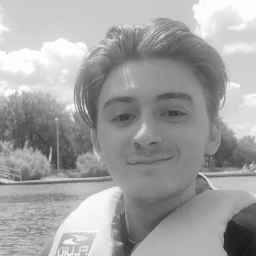
\includegraphics[scale=1.]{./rendus/MOIMOIETMOI.png}}
\caption{Image d'origine}
\end{figure}

\newpage
\section{Création de la carte de gradient d'une image}
Pour cela on applique à chaque pixel la racine carrée  de la somme des carrés des différence verticales et horizontales.
\begin{figure}[h!]
\centerline{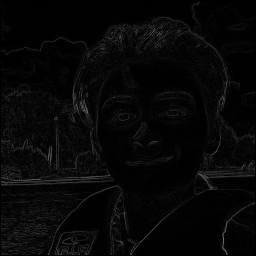
\includegraphics[scale=1.]{./rendus/CartegradientMOI.png}}
\caption{carte de gradient de l'image d'origine}
\end{figure}
\begin{figure}[h!]
\centerline{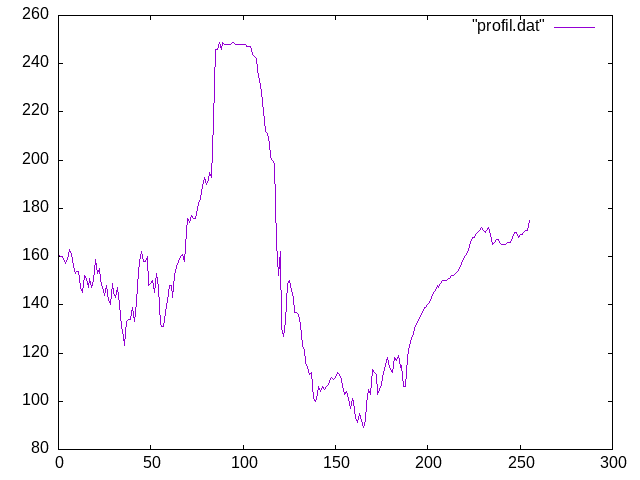
\includegraphics[scale=.5]{./rendus/profil.png}}
\caption{profil de l'image d'origine}
\end{figure}

\newpage
\section{Extraction des maximums locaux par seuillage.}
Seuillage classique
\begin{figure}[h!]
\centerline{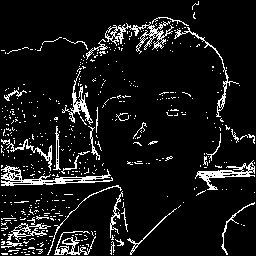
\includegraphics[scale=1.]{./rendus/cartegradientSeuillee.png}}
\caption{carte de gradient de l'image d'origine seuillée}
\end{figure}

\newpage
\section{Seuillage par hystérésis des maximums locaux.}
Le seuillage par hysteresis se fai en 2 passes la première met à 0 les pixels inférieurs au seuil bas et à 255 ceux supérieurs au seuil haut.
Dans la 2e passe on prend ceux entre le seuil bas et le seuil haut et si ils ont dans leurs voisins un pixel à 255 alors ont leur attribue la valeur 255 sinon 0.
\begin{figure}[h!]
\centerline{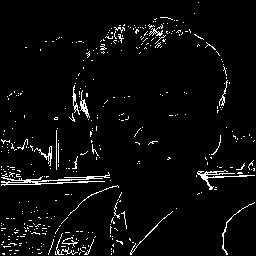
\includegraphics[scale=1.]{./rendus/cartegradientSeuilleeHysteresis.png}}
\caption{carte de gradient de l'image d'origine seuillée avec une seuillage par hystérésis}
\end{figure}

\newpage
\section{Prétraitement par filtrage.}
Pour chaque pixel on lui attribue la moyenne  de ses 8 voisins + lui, donc moyenne de 9 valeurs de pixels.
\begin{figure}[h!]
\centerline{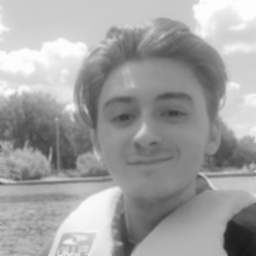
\includegraphics[scale=1.]{./rendus/MOIMOIETMOIfiltree.png}}
\caption{Image d'origine filtree (filtre moyenneur)}
\end{figure}

\begin{figure}[h!]
\centerline{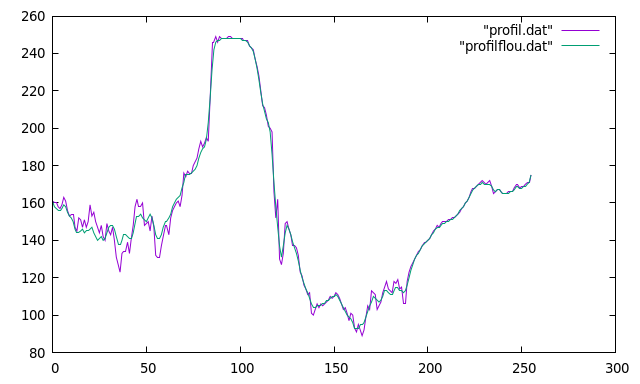
\includegraphics[scale=0.6]{./rendus/profilOriginalEtFloutee.png}}
\caption{Image d'origine filtree (filtre moyenneur)}
\end{figure}

\begin{figure}[h!]
\centerline{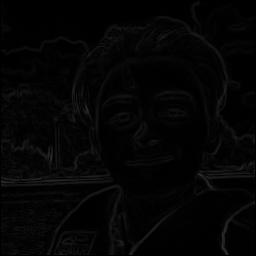
\includegraphics[scale=1.]{./rendus/MOIMOIETMOIfiltreegradient.png}}
\caption{Image d'origine filtree gradient}
\end{figure}

\begin{figure}[h!]
\centerline{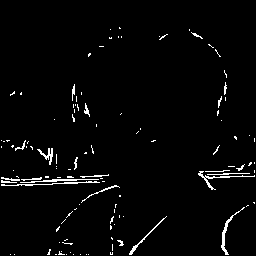
\includegraphics[scale=1.]{./rendus/MOIMOIETMOIfiltreegradientseuille.png}}
\caption{Image d'origine filtree gradient seuillée}
\end{figure}

\begin{figure}[h!]
\centerline{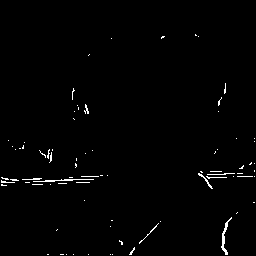
\includegraphics[scale=1.]{./rendus/MOIMOIETMOIfiltreegradientseuillehysteresis.png}}
\caption{Image d'origine filtree gradient seuillée (par hystérésis)}
\end{figure}

\begin{figure}[h!]
\section{Calcul du Laplacien}
Pour chaque pixel, on attribue à ce pixel 4 fois sa valeur + -1 fois * la valeur de ses 4 voisins horizontaux et verticaux, et on ajoute 128 au résultat.

\centerline{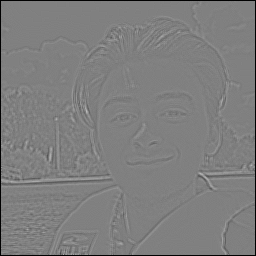
\includegraphics[scale=1.]{./rendus/MOIMOIETMOIfiltreeLaplace.png}}
\caption{Image d'origine filtree et application filtre Laplacien}
\end{figure}


\begin{figure}[h!]
\section{Recherche des passages par zéro}
Pour chaque pixels on calcule applique le filtre Laplacien sans faire +128, ensuite on calcule la direction du gradient, de là on en déduit l'angle de la direction. Celui-ci nous dit avec quel voisin on doit comparer notre pixel, si le pixel courant et notre voisin trouvé on des signes opposés alors on attribue à notre pixel courant la valeur de la norme du gradient.

\centerline{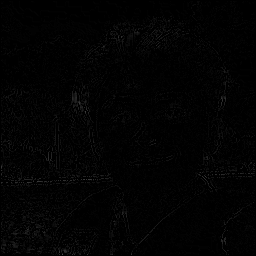
\includegraphics[scale=1.]{./rendus/MOIMOIETMOIfiltreePassagepar0.png}}
\caption{Image d'origine filtree et application filtre Laplacien}
\end{figure}

\begin{figure}[h!]
\section{Recherche des passages par zéro et seuillage par hystérésis}

\centerline{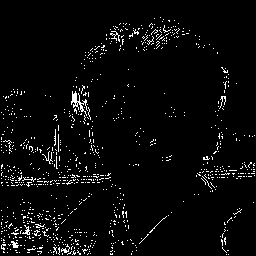
\includegraphics[scale=1.]{./rendus/MOIMOIETMOIfiltreePassagepar0Hysteresis.png}}
\caption{Image d'origine filtree et application filtre Laplacien}
\end{figure}


\end{document}